\documentclass[a4paper,12pt]{article}
\usepackage[utf8]{inputenc}
\usepackage{tocloft}
\usepackage[]{nomencl}
\usepackage{pdfpages}
\usepackage{scrextend}
\usepackage{bm}
\usepackage{cite}
\usepackage{amsmath}
\usepackage{graphicx}
\usepackage[justification=centering]{caption}
\usepackage{float}
\usepackage{multicol}
\usepackage{float}
\usepackage[section]{placeins}
%bindet die benutzten Packages ein

\renewcommand*\vec[1]{\boldsymbol{#1}}
\renewcommand*\matrix[1]{\boldsymbol{#1}}

%setzt die fettgedruckte Schreibweise fuer Vektoren und Matrizen

%opening
\title{Investigations on one-way coupling effects of particle-laden decaying isotropic turbulent flows}
\author{Julian Stemmermann, Steffen Trienekens, Christian Soika}
\date{Aachen, 3rd of July 2017}

%schreibt die generellen Informationen aus

\numberwithin{equation}{section} %bestimmt die Nummerierung der Gleichungen, in diesem Fall nach Kapitel anstatt sie einfach durchzunummerieren

\makenomenclature %erstellt und druckt die Nomenklatur-Tabelle

\renewcommand{\refname}{}
\renewcommand{\nomname}{}

\begin{document}

\maketitle

\setlength{\columnsep}{30pt}

\pagebreak

\tableofcontents{} %erstellt die Inhaltsangabe
 
\pagebreak

\section{Nomenclature}
\begin{multicols}{2}
\setlength{\columnseprule}{1pt}
\printnomenclature
\end{multicols}
\pagebreak

\section{Introduction}
in Computational Methods for Multiphase Flow ist auf den Seiten 3-9 ein interessantes Beispiel.
Sollen wir hier außerdem noch ein Bild von einer turbulenten Strömung und der Sammlung der Partikel in low-vortex-areas einfügen?
Unterschiedliche Sections erklären
Einführung von $m_c$ beschreiben. 
Ablauf:
1. Beispiel für technische Anwendungen
2. Inhalt der Arbeit zusammenfassen
\pagebreak
\section{Mathematical models}
\subsection{Single-phase flow} %Christian
In this section the mathematical basics for understanding and simulating turbulent flows are discussed. However, it should be pointed out that this is no
complete treatise of the mathematical and physical basics. The reader can achieve further insight on this topic by looking at different books and papers, 
e.g. \cite{turbulentFlows}.
\newline
\subsubsection{The Navier-Stokes equations}
The Navier-Stokes-Equations are of great importance for understanding turbulent phenomena. This set of equations exists in forms for compressible and
incompressible fluids. For an infinitesimal small volume element $ \mathrm{d} \tau $ and using the cartesian coordinate system, 
they can be written in the so-called 'divergence form':
\nomenclature{$\vec\nabla$}{Nabla-operator} %Erstellt automatisch die Nomenclature-Liste
\nomenclature{$\vec{Q}$}{Container for conserved variables in the Navier-Stokes equations}
\nomenclature{$\vec{H}$}{Container for fluctuating variables in the Navier-Stokes equations}
\begin{equation}
  \frac{\partial{\vec{Q}}}{\partial{t}} + \vec\nabla \vec{H} = 0
\end{equation}
The vector $ \vec{Q} $ contains all the variables which are conserved, i.e. the density $ \rho $, 
the velocity $ \vec{u} $ and the specific inner energy $ E $: 
\nomenclature{$\rho$}{Density}
\nomenclature{$\vec{u}$}{Three-dimensional velocity}
\nomenclature{$E$}{Specific inner energy}
\begin{equation}
 \vec{Q}= \left( \begin{array}{c}\rho\\\rho \vec{u}\\\rho E \end{array} \right)
\end{equation}
$ \vec{H} $ is the flux vector which stores all the floating variables and may be split up into two parts:
\nomenclature{$\vec{H^\mathrm{i}}$}{Stores the inviscid variables in the flux-vector included in the Navier-Stokes equations}
\nomenclature{$\vec{H^\mathrm{v}}$}{Stores the viscous variables in the flux-vector included in the Navier-Stokes equations} 
\begin{equation}
 \vec{H} = \vec{H^\mathrm{i}} + \vec{H^\mathrm{v}}
\end{equation}
The contents of the two vectors are displayed below:
\nomenclature{$p$}{Pressure}
\nomenclature{$Re$}{Reynolds number}
\nomenclature{$\matrix{\tau}$}{Stress tensor}
\nomenclature{$\vec{q}$}{Heat conduction}
\begin{equation}
 \vec{H^\mathrm{i}} = \left( \begin{array}{c}\rho \vec{u}\\\rho \vec{u} \vec{u} + p\\\vec{u} (\rho E + p) \end{array} \right)
\end{equation}
\begin{equation}
 \vec{H^\mathrm{v}} = - \frac{1}{Re} \left( \begin{array}{c}\ 0 \\ \matrix{\tau}\\ \matrix{\tau} \vec{u} + \vec{q} \end{array} \right)
\end{equation}
$ \vec{H^\mathrm{i}} $ is called inviscid flux and contains only the variables that are independent of the fluids viscosity, it describes the way a fluid 
with zero viscosity would behave. In contrast, the viscous flux $ \vec{H^\mathrm{v}} $ represents the effects of viscosity. The Reynolds number 
$ Re = \frac{\rho v d}{\eta} $ is defined to be the ratio of inertia to tenacity, which makes it very valuable for understanding turbulent flows. This is also due to the 
fact that two familiar objects with the same Reynolds number behave similar in turbulence. One can assume that flows with $ Re << 1 $ are laminar and flows with 
$ Re >> 1 $ are turbulent.
To solve the Navier-Stokes-Equations, more information regarding some variables is required. For Calculating the specific inner Energy $ E $ 
and the heat conduction $ \vec{q} $, the following equations are used:
\nomenclature{$e$}{Specific internal energy}
\nomenclature{$Pr$}{Prandtl number}
\nomenclature{$\mu$}{Dynamic viscosity}
\begin{equation}
 E = e  \frac{1}{2} \vec{|u|}^2
\end{equation}
\begin{equation}
 \vec{q} = - \frac{\mu}{Pr (\gamma - 1)} \vec\nabla T
\end{equation}
with 
\nomenclature{$c_p$}{Specific isobaric heat capacity}
\nomenclature{$c_v$}{Specific isochoric heat capacity}
\begin{equation}
 \gamma = \frac{c_p}{c_v}
\end{equation}
and the Prandtl number
\nomenclature{$k_t$}{thermal conductivity}
\begin{equation}
 Pr = \frac{\mu_\infty c_p}{k_t}
\end{equation}
using the specific heat capacities of the fluid $ c_v $ and $ c_p $.
If one could assume that the fluid is a newtonian fluid, the linear correlation between stress and the rate of strain results in:
\nomenclature{$\matrix{I}$}{Identity tensor}
\nomenclature{$\matrix{S}$}{Rate-of-strain-tensor}
\nomenclature{$T$}{Temperature}
\begin{equation}
 \matrix{\tau} = 2 \mu \matrix{S} - \frac{2}{3} \mu (\vec\nabla * \vec{u}) \matrix{I}
\end{equation}
in which $ \matrix{S} = \frac{(\vec\nabla \vec{u})(\vec\nabla \vec{u})^T}{2} $ denotes the rate-of-strain-tensor. Additionally, the viscosity
$ \mu $ can be aprroximated through Sutherland's law, which is based on the ideal gas-theory: 
\nomenclature{$S$}{Sutherland temperature}
\nomenclature{$R$}{Universal gas constant}
\begin{equation}
 \mu (T) = \mu_\infty (\frac{T}{t_\infty})^{3/2} \frac{T_\infty + S}{T + S}
\end{equation}
S is in this case the Sutherland temperature.
To achieve closure the caloric state equation $ e = c_v T $ and the state eqaution for an ideal gas $
p = \rho R T $ are used. The specific gas constant is determined by $ R = c_p - c_v $. 
These equations form a set of partial differential equations, so for solving them starting values are needed.
\pagebreak
\subsection{Particle dynamics} %Steffen
Siewert:
-3.1a-3.14 (spherical particles) OHNE GRAVITATION
Stokes Drag/Stokes Coefficient
Filterung (Fritz) ->Viskositaet durch numerischen Fehler, Smagorinksy nicht benutzen
\newline
\newline
Cause this work deals with particle laden fluids and the impact of these particles on the flow conditions, we need to describe the interaction between them. 
We deal with small and heavy, rigid particles, that have a spherical shape. Their radius $ r_p $ is even smaller than the Kolmogorov scale $ \eta $, but also large enough to neglect the Brownian motion.
Due to the small particle concentration, the best and most common way to describe these flows is the point particle approach, which means that every particle is treated as an mathematical point source of mass, momentum and energy. In this case we focus on the momentum exchange.Effects like particle-particle interactions, particle-wall interactions are also neglected.  
At describing the motion of the particles in the following the fact, that we deal with gas-solid flows is an advantage, since we can make several simplifications.
First we look at the influence of the particles on the carrier fluid. Here we make the assumption, that the fluid is incompressible and the mass exchange over the particle surface is zero.
Hence the continuity equation becomes:
\begin{equation}
dreieck * \vec{u}
\end{equation}.
The Navier Stokes equation, described in chapter 1, becomes:
\begin{equation}
\rho*(-F)
\end{equation}
The influence of the particles on the fluid is represented by the new term F, wich describes the force per unit volume on the fluid.
We could approximate F by a superposition of Dirac's delta functions over all particles, centered at the location $x_p^n$ of each particle:
\begin{equation}
F = f^n
\end{equation}
$\vec{x_\mathrm{p}^\mathrm{n}} $ is the position of the n-th particle and results from the kinematic equation 
\begin{equation}
 \frac{\partial{\vec{x_\mathrm{p}}}}{\partial{t}} = \vec{v_\mathrm{p}}
\end{equation}
$\vec{v_\mathrm{p}}$ is the velocity of the n-th particle.
$\vec{f^\mathrm{n}}$ is the sum of forces acting between fluid an particles.
Hence it plays also an important role in the equation of motion of the particles:
\begin{equation}
v_v*\rho_p* \frac{\partial{\vec{v_\mathrm{p}^\mathrm{n}}}}{\partial{t}} = v_v*\rho_\mathrm{p}*\vec{g}+\vec{f^\mathrm{n}(\vec{x_\mathrm{p}^\mathrm{n}})}
\end{equation}
As already mentioned $\vec{f^\mathrm{n}(\vec{x_\mathrm{p}^\mathrm{n}})}$ could be devided in several forces. Then the equation of motion looks like:
\begin{equation}
v_v*\rho_p* \frac{\partial{\vec{v_\mathrm{p}^\mathrm{n}}}}{\partial{t}} = v_v*\rho_\mathrm{p}*\vec{g}+\vec{f_\mathrm{d}}+\vec{f_\mathrm{l}}+\vec{f_\mathrm{a}}+\vec{f_\mathrm{h}}+\vec{f_\mathrm{additional}}
\end{equation}
Here $\vec{f_\mathrm{d}}$ represents the hydrodynamical drag force that is parallel to the undisturbed streamlines, which depends on an empirical drag coefficient $C_{\mathrm{d}} $:
\begin{equation}
\vec{f_\mathrm{d}}=-\frac{3}{4}*\rho*v_\mathrm{v}*\frac{C_\mathrm{d}}{d}*|\vec{v_\mathrm{p}}-\vec{u}|*(\vec{v_\mathrm{p}}-u)
\end{equation}
$\vec{u}$ is the velocity of the uniform stream, which is enough away from the particle that it is undisturbed from the particle.
The other partial hydrodynamical force, the lift force $\vec{f_\mathrm{l}}$ is perpendicular to the undisturbed streamlines.
Furthermore the added mass force $\vec{f_\mathrm{a}}$ represents the influence of the inertia of the fluid that has an impact on the particle, if it has a different acceleration than the mean flow.
Hence it could be determined by:
\begin{equation}
\vec{f_\mathrm{a}} =  \frac{1}{2}*\rho*v_\mathrm{v}*(\frac{D*\vec{u}}{D*t}-\frac{d*\vec{v_\mathrm{p}}}{d*t})
\end{equation}
-------nie $\vec{v}$ sondern immer $\vec{v_\mathrm{p}}$ benutzen-----------
The history force $\vec{f_\mathrm{h}}$ takes diffusion and convection, that results out of the vortices behind the particles, into account. We look at Basselt's result, neglecting the finite size correction that is proportional to $\vec\nabla^\mathrm{2}*\vec{u}$:
\begin{equation}
\vec{f_\mathrm{h}} = \frac{3}{2}*d^\mathrm{2}*\rho*\sqrt{\pi*\nu}*\int_t\mathrm{0}^t \frac{\mathrm{d}t'}{(t-t')^\mathrm{1/2}} (\frac{\mathrm{D}\vec{u}}{\mathrm{D}t'}- \frac{\mathrm{d}\vec{v_\mathrm{p}}}{\mathrm{d}t'}) \, 
\end{equation}
In our case of gas-solid suspensions we can make several simplifications.
In the following we show with an rough approximation that the added mass and history forces are negligible compared with the drag force.
We use the approach that the relative velocity is of the same order as the terminal velocity $v_\mathrm{t}$. The terminal velocity is the velocity of a particle in a resting fluid, when gravitation and drag force are in equilibrium. Then if the added mass and the drag force are compared, we get the following equation:
\begin{equation}
\frac{|\vec{f_\mathrm{a}}|}{|\vec{f_\mathrm{d}}} \simeq \approx \frac{\frac{1}{2}*\rho*v_\mathrm{v}*g}{\frac{3}{4}*\rho*v_\mathrm{v}*(C_\mathrm{d}/d)*v_\mathrm{t}^\mathrm{2}}\frac{a_\mathrm{r}}{g} = \frac{1}{2}*\frac{\rho}{\rho_\mathrm{p}}*\frac{a_\mathrm{r}}{g}
\end{equation}
with 
\begin{equation}
a_\mathrm{r}=(\frac{\mathrm{D}\vec{u}}{\mathrm{d}t}-\frac{\mathrm{d}\vec{v_\mathrm{p}}}{\mathrm{d}t})
\end{equation}
Since in gas-solid suspensions the particle density is of an factor of 1000 higher than the fluid density, it shows that, if it's not the unlikely case that the relative acceleration is of the same order higher than the gravity, the added mass force is negligible compared to the drag force.
The effect that fluid and particle influence each other is called two-way-coupling.
$\vec{f_\mathrm{d}}$ and lift forces, $\vec{f_\mathrm{a}}$  the added mass and $\vec{f_\mathrm{h}}$ the history forces. The last term $\vec{f_\mathrm{additional}}$ is attached for the case that we have to take other forces like electrostatic interactions into account.
\newline
-coupling Zahl
\newline
The relaxation time $\tau_\mathrm{p}$ physically represents the time scale over which the drag force decreases the particle relative veloctity to zero and is determined by the following equation:
\begin{equation}
\tau_\mathrm{p} = \frac{rho_\mathrm{p}}{rho}*\frac{2*r_\mathrm{p}^\mathrm{2}}{9*\nu}
\end{equation}
Since we consider gas-solid flows, wich means  we can use a point particle approach  make some simplificantions in the following 
To get a usefull equation of motion for the particles in the flow, we use the Euler Lagrangian approach, as it is common in Direct Numerical Simulations (DNS) and Large Eddy Simulations (LES).
 The density of the particles $ \rho_\mathrm{p} $ is much higher than that of the fluid $ \rho_\mathrm{f} $ . 
In addition due to the very low particle concentration we can neglect the influence of the particles on each other. That means that the cross each other without any effect. That means particle collision is neglected.
After all this simplifications we obtain a simplified version of the Maxey-Riley equations. 
\nomenclature{$r_p$}{Particle radius}
\nomenclature{$\eta$}{Kolomogorov scale}
\nomenclature{$\rho_\mathrm{p}$}{Particle density}
\begin{equation}
 \frac{\partial{\vec{x_\mathrm{p}}}}{\partial{t}} = \vec{v_\mathrm{p}}
\end{equation}
\nomenclature{$\vec{x_\mathrm{p}}$}{Particle position}
\nomenclature{$\vec{v_\mathrm{p}}$}{Particle velocity}
\begin{equation}
 \frac{\partial{\vec{v_\mathrm{p}}}}{\partial{t}} = \frac{f_mathrm{D}}{tau_mathrm{p}} (\vec{u(x_\mathrm{p}}) - \vec{v_\mathrm{p}})
 \end{equation}
 \nomenclature{$f_mathrm{D}$}{Drag correction}
 \nomenclature{$\tau_mathrm{p}$}{Particle response time}
%It shows that the particle motion is only depending on the the hydrodynamical drag force which results out of the actual difference between the fluid velocity $\var{u(x_\mathrm{p})}$ at particle position $\var{x_p}$ and the particle velocity $\var{v_p}$.
 $\tau_mathrm{p}$ is the particle response time and a factor to obtain the drag force in Stokes flow conditions.
 To take the case of an Reynolds number $\Re$ of order 1 into account the correction factor $f_D = 1 + 0.15 Re_p^(0.687)$ is used.
 The biggest simplification of this Lagrangian approach is that the interaction of particles coming close together is neglected. 
 \pagebreak
\section{Numerical methods} %Julian
To simulate flows like those described above we have two options. The direct numerical simulation (DNS) is the easier one to understand, although it is numerically very expensive. The Large-eddy simulation (LES) is numerically more capable, still we must accept certain inaccuracies. These two numerical methods are now discussed in the following chapter.
\subsection{Direct numerical simulation}
The basis of the direct numerical simulation (DNS) are the Navier-Stokes equations as described above. The idea is that the computer is very good at calculating and solves these equations completely. This provides a very accurate result, as all scales of motion are being resolved. Still it requires an immense level of comptational resources which increases rapidly with the Reynolds number. These computational resources were not available until the 1970s. Even though it is not advisable to resolve every scale of motion, if only the contained energy is of greatest interest. With the large-eddy simulation, as described below, the comptational effort is 99.98 \% less compared to DNS, which indeed is the fraction of the dissipative scale. This leaves 0.02 \% of the flow, which is correlative with the fraction of the energy-containing larger-scale \cite{turbulentFlows}.%zum Uebergang zu LES siehe Pope S. 352 und Fig. 9.4
\subsection{Large-eddy simulation}
Due to the fact that DNS is effortful and wasting resources if a fully resolved resolution is not required, large-eddy simulation (LES) was created to save time and resources. This is especially efficient if mainly the temproal energy trend is considered, because the energy containing larger-scale motion is completely resolved and the indeed small effects of the expensive smaller-scale motion are just modelled. Otherwise in DNS resolving the small dissipative scale would require most of the computational resources.
\newline
Simulating only the larger-scale motions is also called filtering, which means that the smaller-scale motions are filtered out. To model the filtered smaller-scale motions ususally a subgrid-scale (SGS) model is used. According to Hickel (2007) the interference between explicit SGS and the trunctation error can be exploited, i.e. the trunctation error can serve as model of the effects of unresolved scales, which is therefore an implicit SGS model. Thus we call it implicit LES (ILES) \cite{implicitLES}. %als Zitat die Dissertation TUM Hickel
\subsection{Discretisation}
To integrate the Lagrangian particle tracking equations, discussed above, a predictor-corrector scheme based on the trapezoidal rule for numerical integration
\begin{equation}
f (t + \delta t) \approx f(t) + \frac{\delta t}{2} \left[ \frac{\partial f(t)}{\partial t} + \frac{\partial f(t + \delta t)}{\partial t} \right ]
\end{equation}
is used.
\newline
The first step is the prediction of the new particle position $\vec{x}_{n+1}^\mathrm{(p)}$ using a Taylor expansion for a small time step $\delta t$
\nomenclature{$\vec{x}$}{particle position}% ++ nomenclature funktioniert noch nicht! ++
\nomenclature{$\vec{v}$}{particle velocity}% ++ nomenclature funktioniert noch nicht! ++
\nomenclature{$\vec{a}$}{particle acceleration}% ++ nomenclature funktioniert noch nicht! ++
\begin{equation}
\vec{x}_{n+1}^\mathrm{(p)} = \vec{x}_n + \delta t \vec{v}_n + \frac{1}{2} \delta t^2 \vec{a}_n.
\end{equation}
Due to the computational effort we will put $\vec{u}_{n+1}^\mathrm{(p)}$ on the level of the nearest cell fluid velocity.
\newline
The updated velocity and acceleration are calculated as
\begin{equation}
\vec{v}_{n+1} = \frac{\vec{v}_n + \frac{1}{2} \delta t \left(\vec{a}_n + \frac{f_\mathrm{D}}{\tau_\mathrm{p}}\vec{u}_{n+1}^\mathrm{(p)} + \vec{g} \right)}{1 + \frac{1}{2} \frac{f_\mathrm{D}}{\tau_\mathrm{p}} \delta t},
\end{equation}
\begin{equation}
\vec{a}_{n+1} = \frac{\frac{f_\mathrm{D}}{\tau_\mathrm{p}} \left(\vec{u}_{n+1}^\mathrm{(p)} - \vec{v}_n - \frac{1}{2} \delta t \vec{a}_n \right) + \vec{g}}{1 + \frac{1}{2} \frac{f_\mathrm{D}}{\tau_\mathrm{p}} \delta t}.
\end{equation}
The updated particle position must be corrected by an additional term according to the trapezoidal rule
\begin{equation}
\vec{x}_{n+1} = \vec{x}_n + \frac{1}{2} \delta t \left( \vec{v}_{n+1} + \vec{v}_{n} \right) + \frac{1}{12} \delta t^2 \left( \vec{a}_{n+1} - \vec{a}_n \right).
\end{equation}
\subsection{Particle clustering}
\nomenclature{$m_\mathrm{c}$}{number of clustered particles}% ++ nomenclature funktioniert noch nicht! ++
The high number of point particles require even more computational resources for the particle-laden simulation. The main idea to reduce this requirement is to create clusters of point particles, meaning that a new variable $m_\mathrm{c}$ is introduced. We consider a cluster of $m_\mathrm{c}$ point particles as one larger point particle, i.e. the program has less particles to simulate. To compensate this lack of particles, the coupling force is multiplied by $m_\mathrm{c}$, due to the $m_\mathrm{c}$-fold mass of the (cluster-)particles. In chapter 5 (results) we evaluate the legitimacy of particle clustering and the maximum acceptable value of $m_\mathrm{c}$.
\newline
\newline
Projektion (noComputationalParticles), Diskretisierung
implizite LES (Motivation fuer LES -  Pope Chapter 9, Bild 9.4), DNS
\pagebreak
\section{Results}
The simulations where carried out using ZFS, the simulation tool developed and implemented at the Institute of Aerodynamics at RWTH Aachen University 
\cite{anAdaptiveMultilevelMultigridFormulationForCartesianHierarchicalGridMethods} \cite{aStrictlyConservativeCartesianCutCellMethodForCompressibleViscousFlowsOnAdaptiveGrids}. 
The tool is capable of simulating finite-volume flows of compressible fluids. 
In this case the turbulence was simulated on a cubic grid using $64^3$,$96^3$,$128^3$ and $256^3$. The first three cases where simulated using LES, 
the case in which $256^3$ cells where used is carried out as DNS. Futher information can be gained by looking at \cite[p.344-357 for DNS and p. 558-639 for LES]{turbulentFlows}.
\begin{figure}[h]
	\centering
  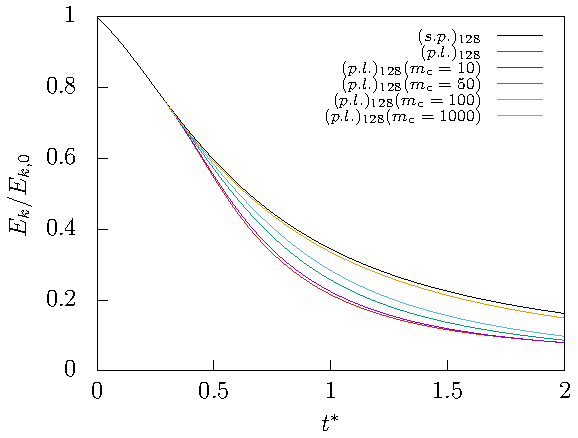
\includegraphics[width=0.9\textwidth]{./../Simulationsergebnisse/variationWolken/128/kineticEnergy_time.pdf}
	\caption{Kinetic Energy over time for different numbers of particles}
	\label{kineticEnergy_time_128}
\end{figure}
\newline
For simplification, the special case of isotropic turbulence was used. For this idealised flow form the statistical 
velocities are invariant in all directions of the grid. It follows that the flows velocity are invariant for rotations and reflections. 
The turbulence was initialised using a seed-based random generator. To achieve physical results, the simulation of the particle-free flow was carried out  to timestep 150, 
at which a restart file was written out. This procedure ensures a fully developed turbulent 
flow, whom has emancipated from the initialisation. In this flow field, a specific number of spherical particles were injected. 
\nomenclature{$m_\mathrm{c}$}{Number of particles in a particle cluster}
\newline
As noted in \cite{PreferentialConcentrationOfHeavyParticles}, particles tend to cluster in certain regions of the turbulent flow. This behavior can bee used to minimize computational effort for simulating the flow while still achieving high quality results. To investigate the differences in accuracy for different sizes of particles sizes, the variable $m_\mathrm{c}$ was introduced to the code describing the number of particles in one cluster. The simulations where then set up with the overall same number of particles ($ 10^6 $), just the number of particles in one cluster was altered. Then the simulations where carried out normally and result in the following graphs (Figure \ref{kineticEnergy_time_128}, \ref{der(kineticEnergy)_time_128} and \ref{coupling_time_128}). 
It can be seen in figure \ref{kineticEnergy_time_128} that the decay in kinetic energy from the starting point depends highly on the number of clustered particles. \textbf{With 10 particles per cluster, the solutions could be usable to get a first impression for technical purposes, all other simulations show a very high variety.}
\newline
\begin{figure}[h]
    \centering
    \begin{minipage}{.5\textwidth}
        \centering
        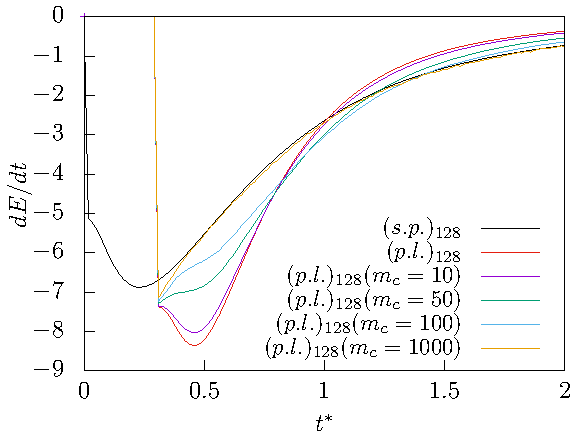
\includegraphics[width=\linewidth]{./../Simulationsergebnisse/variationWolken/128/der(kineticEnergy)_time.pdf}
        \caption{Change in kinetic Energy over normalized time}
        \label{der(kineticEnergy)_time_128}
    \end{minipage}%
    \begin{minipage}{0.5\textwidth}
        \centering
        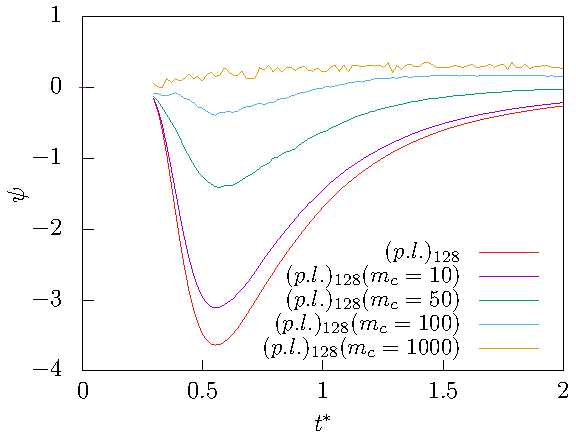
\includegraphics[width=\linewidth]{./../Simulationsergebnisse/variationWolken/128/coupling_time.pdf}
        \caption{Coupling Rate over normalized time}
        \label{coupling_time_128}
    \end{minipage}
\end{figure}
Fitting to this first results, the Graphs of figure \ref{der(kineticEnergy)_time_128} and \ref{coupling_time_128} clearly show that for simulations with highly clustered particles the simulations results differ a lot. Looking at the results for the change in kinetic Energy, the difference becomes evident: The lower $ m_\mathrm{c} $ is, the higher is the drop in kinetic Energy. This behavior can be seen because of the particles initially 'soaking up' energy, then in later phases of the flow giving it back in form of their inertia and speed, which they gathered in the beginning. \textbf{This effect should grow bigger by particle size and weight.} This change in energy transfer occurs at the unclustered simulation at about one eddy turnover time ($t^*$). In cases with more clustered particles it occurs later, only the case in which 1000 particles where clustered shows a strange behavior. It catches up the particle-free case very fast, which leads to the conclusion that the amount of clusters is so small that the flow almost behaves like one without particles. Additional the change in kinetic Energy shows inconstancy which can also be traced back to the small cluster number. The amount is just to small to achieve high-quality information in the statistical variables. 
\newline
The same impression can be achieved by looking at the graphs describing the coupling rate. The particle-laden-case makes the biggest jump into negative coupling rate, which is defined as: \textbf{Defnition Coupling Rate}. The higher the amount of coupled particles, the lower is the negative coupling force. This evolution continues until the physicality vanishes and the randomness starts to show at the results for $m_\mathrm{c}$ higher than 50. 
\newline
The properties of these simulations can be found in table \ref{table_properties} on page \pageref{table_properties}.
\begin{table}[h]
\begin{tabular}{l | c c c c c c c }
Case & $u_0$ & $\epsilon$ & $l$ & $\lambda$ & $\eta $ & $Re_\mathrm{l}$ & $Re_\lambda$ \\
\hline
\hline
64 & 1.50053 & 0.0022661 & ? & 0.0348981 & ? & ? & 41.4212 \\
96 & ? & ? & ? & ? & ? & ? & ? \\
128 & ? & ? & ? & ? & ? & ? & ?  \\
264 & ? & ? & ? & ? & ? & ? & ?  \\
\hline
\end{tabular}
\caption{Properties of the first set of simulations}
\label{table_properties}
\end{table}
\newline
To find out at which number of particles the results are sufficiently exact, a second set of simulations was carried out. As mathematics of turbulent flows are based on averaged variables, small numbers of particles can lead to false and even unphysical results. In these simulations, no particle clustering was used, just different amount of particles were injected into the same flow. For these simulations similar properties to the ones from the first set of simulations were used, just the mentioned number of particles was changed. The results can be seen on page \pageref{kineticEnergy_numberOfParticles} on figure \ref{kineticEnergy_numberOfParticles}. 
\begin{figure}[h]
	\centering
  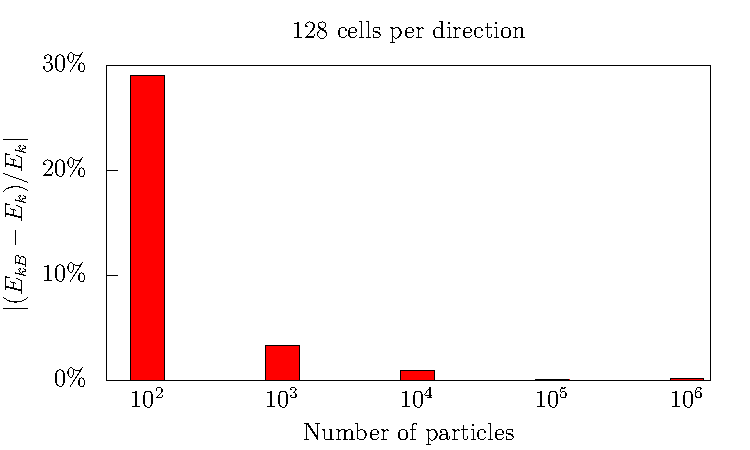
\includegraphics[width=\textwidth]{./../Simulationsergebnisse/variationPartikelAnzahl/128/kineticEnergy_numberOfParticles.pdf}
	\caption{Results for initializing different numbers of particles}
	\label{kineticEnergy_numberOfParticles}
\end{figure}
The normalized difference in \textbf{kinetic Energy} shows as expected a clear correlation between particle number and accuracy in the simulation. Athough this was just a single initialization of particles in a flow, it can be stated that simulations using only $10^2$, $10^3$ or even up to $10^4$ particles are not accurate enough for technical or scientific use of the data. Simulations in other gridsizes show similar results.
\pagebreak
\section{Conclusion}
\subsection*{Acknowledgements}
\pagebreak
\section{References}
\nocite{*} %ermoeglicht, dass auch Literatur, welche nicht zitiert wurde in der Bibliography auftaucht
\bibliography{Projektarbeit} %ruft die Bibliography-Datei auf
\bibliographystyle{plain} %setzt den Zitierstil
\pagebreak
\end{document}
